% Options for packages loaded elsewhere
\PassOptionsToPackage{unicode}{hyperref}
\PassOptionsToPackage{hyphens}{url}
\PassOptionsToPackage{dvipsnames,svgnames,x11names}{xcolor}
%
\documentclass[
  letterpaper,
  DIV=11,
  numbers=noendperiod]{scrartcl}

\usepackage{amsmath,amssymb}
\usepackage{iftex}
\ifPDFTeX
  \usepackage[T1]{fontenc}
  \usepackage[utf8]{inputenc}
  \usepackage{textcomp} % provide euro and other symbols
\else % if luatex or xetex
  \usepackage{unicode-math}
  \defaultfontfeatures{Scale=MatchLowercase}
  \defaultfontfeatures[\rmfamily]{Ligatures=TeX,Scale=1}
\fi
\usepackage{lmodern}
\ifPDFTeX\else  
    % xetex/luatex font selection
\fi
% Use upquote if available, for straight quotes in verbatim environments
\IfFileExists{upquote.sty}{\usepackage{upquote}}{}
\IfFileExists{microtype.sty}{% use microtype if available
  \usepackage[]{microtype}
  \UseMicrotypeSet[protrusion]{basicmath} % disable protrusion for tt fonts
}{}
\makeatletter
\@ifundefined{KOMAClassName}{% if non-KOMA class
  \IfFileExists{parskip.sty}{%
    \usepackage{parskip}
  }{% else
    \setlength{\parindent}{0pt}
    \setlength{\parskip}{6pt plus 2pt minus 1pt}}
}{% if KOMA class
  \KOMAoptions{parskip=half}}
\makeatother
\usepackage{xcolor}
\setlength{\emergencystretch}{3em} % prevent overfull lines
\setcounter{secnumdepth}{-\maxdimen} % remove section numbering
% Make \paragraph and \subparagraph free-standing
\ifx\paragraph\undefined\else
  \let\oldparagraph\paragraph
  \renewcommand{\paragraph}[1]{\oldparagraph{#1}\mbox{}}
\fi
\ifx\subparagraph\undefined\else
  \let\oldsubparagraph\subparagraph
  \renewcommand{\subparagraph}[1]{\oldsubparagraph{#1}\mbox{}}
\fi


\providecommand{\tightlist}{%
  \setlength{\itemsep}{0pt}\setlength{\parskip}{0pt}}\usepackage{longtable,booktabs,array}
\usepackage{calc} % for calculating minipage widths
% Correct order of tables after \paragraph or \subparagraph
\usepackage{etoolbox}
\makeatletter
\patchcmd\longtable{\par}{\if@noskipsec\mbox{}\fi\par}{}{}
\makeatother
% Allow footnotes in longtable head/foot
\IfFileExists{footnotehyper.sty}{\usepackage{footnotehyper}}{\usepackage{footnote}}
\makesavenoteenv{longtable}
\usepackage{graphicx}
\makeatletter
\def\maxwidth{\ifdim\Gin@nat@width>\linewidth\linewidth\else\Gin@nat@width\fi}
\def\maxheight{\ifdim\Gin@nat@height>\textheight\textheight\else\Gin@nat@height\fi}
\makeatother
% Scale images if necessary, so that they will not overflow the page
% margins by default, and it is still possible to overwrite the defaults
% using explicit options in \includegraphics[width, height, ...]{}
\setkeys{Gin}{width=\maxwidth,height=\maxheight,keepaspectratio}
% Set default figure placement to htbp
\makeatletter
\def\fps@figure{htbp}
\makeatother

\KOMAoption{captions}{tableheading}
\makeatletter
\makeatother
\makeatletter
\makeatother
\makeatletter
\@ifpackageloaded{caption}{}{\usepackage{caption}}
\AtBeginDocument{%
\ifdefined\contentsname
  \renewcommand*\contentsname{Table of contents}
\else
  \newcommand\contentsname{Table of contents}
\fi
\ifdefined\listfigurename
  \renewcommand*\listfigurename{List of Figures}
\else
  \newcommand\listfigurename{List of Figures}
\fi
\ifdefined\listtablename
  \renewcommand*\listtablename{List of Tables}
\else
  \newcommand\listtablename{List of Tables}
\fi
\ifdefined\figurename
  \renewcommand*\figurename{Figure}
\else
  \newcommand\figurename{Figure}
\fi
\ifdefined\tablename
  \renewcommand*\tablename{Table}
\else
  \newcommand\tablename{Table}
\fi
}
\@ifpackageloaded{float}{}{\usepackage{float}}
\floatstyle{ruled}
\@ifundefined{c@chapter}{\newfloat{codelisting}{h}{lop}}{\newfloat{codelisting}{h}{lop}[chapter]}
\floatname{codelisting}{Listing}
\newcommand*\listoflistings{\listof{codelisting}{List of Listings}}
\makeatother
\makeatletter
\@ifpackageloaded{caption}{}{\usepackage{caption}}
\@ifpackageloaded{subcaption}{}{\usepackage{subcaption}}
\makeatother
\makeatletter
\@ifpackageloaded{tcolorbox}{}{\usepackage[skins,breakable]{tcolorbox}}
\makeatother
\makeatletter
\@ifundefined{shadecolor}{\definecolor{shadecolor}{rgb}{.97, .97, .97}}
\makeatother
\makeatletter
\makeatother
\makeatletter
\makeatother
\ifLuaTeX
  \usepackage{selnolig}  % disable illegal ligatures
\fi
\IfFileExists{bookmark.sty}{\usepackage{bookmark}}{\usepackage{hyperref}}
\IfFileExists{xurl.sty}{\usepackage{xurl}}{} % add URL line breaks if available
\urlstyle{same} % disable monospaced font for URLs
\hypersetup{
  pdftitle={Exam 1 Review},
  colorlinks=true,
  linkcolor={blue},
  filecolor={Maroon},
  citecolor={Blue},
  urlcolor={Blue},
  pdfcreator={LaTeX via pandoc}}

\title{Exam 1 Review}
\author{}
\date{}

\begin{document}
\maketitle
\ifdefined\Shaded\renewenvironment{Shaded}{\begin{tcolorbox}[enhanced, frame hidden, interior hidden, breakable, borderline west={3pt}{0pt}{shadecolor}, boxrule=0pt, sharp corners]}{\end{tcolorbox}}\fi

In 2020, employees of Blizzard Entertainment circulated a spreadsheet to
anonymously share salaries and recent pay increases amidst rising
tension in the video game industry over wage disparities and executive
compensation. (Source:
\href{https://www.bloomberg.com/news/articles/2020-08-03/blizzard-workers-share-salaries-in-revolt-over-wage-disparities}{Blizzard
Workers Share Salaries in Revolt Over Pay})

The name of the data frame used for this analysis is
\texttt{blizzard\_salary} and the relevant variables are:

\begin{itemize}
\item
  \texttt{percent\_incr}: Raise given in July 2020, as percent increase
  with values ranging from 1 (1\% increase to 21.5 (21.5\% increase)
\item
  \texttt{salary\_type}: Type of salary, with levels \texttt{Hourly} and
  \texttt{Salaried}
\item
  \texttt{annual\_salary}: Annual salary, in USD, with values ranging
  from \$50,939 to \$216,856.
\item
  \texttt{performance\_rating}: Most recent review performance rating,
  with levels \texttt{Poor}, \texttt{Successful}, \texttt{High}, and
  \texttt{Top}. The \texttt{Poor} level is the lowest rating and the
  \texttt{Top} level is the highest rating.
\end{itemize}

The top six rows of \texttt{blizzard\_salary} are shown below:

\begin{verbatim}
# A tibble: 409 x 4
   percent_incr salary_type annual_salary performance_rating
          <dbl> <chr>               <dbl> <chr>             
 1          1   Salaried               1  High              
 2          1   Salaried               1  Successful        
 3          1   Salaried               1  High              
 4          1   Hourly             33987. Successful        
 5         NA   Hourly             34798. High              
 6         NA   Hourly             35360  <NA>              
 7         NA   Hourly             37440  <NA>              
 8          0   Hourly             37814. <NA>              
 9          4   Hourly             41101. Top               
10          1.2 Hourly             42328  <NA>              
# i 399 more rows
\end{verbatim}

\hypertarget{question-1}{%
\subsection{Question 1}\label{question-1}}

How rows observations are there in the \texttt{blizzard\_salary} dataset
and what does each row represent?

\(\vspace{2cm}\)

\hypertarget{question-2}{%
\subsection{Question 2}\label{question-2}}

Figure~\ref{fig-blizzard-hist-1} and Figure~\ref{fig-blizzard-hist-2}
show the distributions of annual salaries of hourly and salaried
workers. The two figures show the same data, with the facets organized
across rows and across columns. Which of the two figures is better for
comparing the median annual salaries of hourly and salaried workers.
Explain your reasoning.

\begin{figure}

{\centering 

\begin{figure}

{\centering 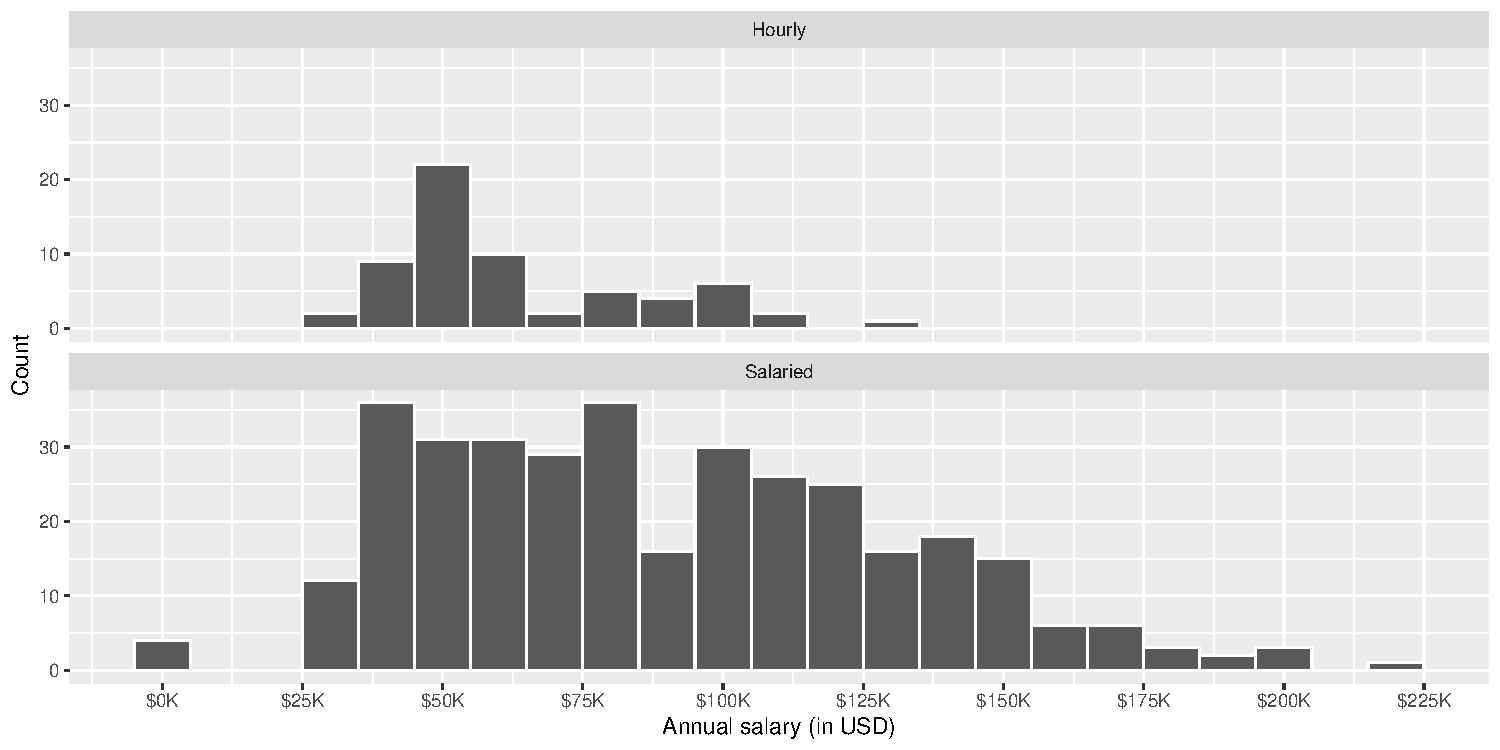
\includegraphics{exam-1-review_files/figure-pdf/fig-blizzard-hist-1-1.pdf}

}

\caption{Option 1}

\end{figure}

\begin{figure}

{\centering 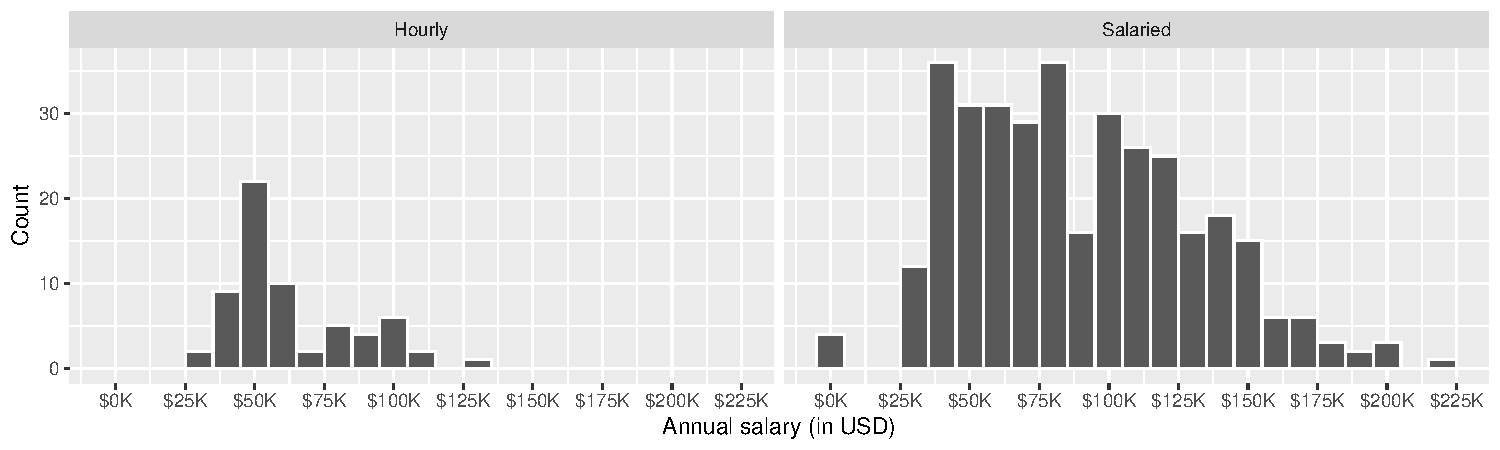
\includegraphics{exam-1-review_files/figure-pdf/fig-blizzard-hist-2-1.pdf}

}

\caption{Option 2}

\end{figure}

}

\caption{\label{fig-blizzard-hist}Distribution of annual salaries of
Blizzard employees}

\end{figure}

\(\vspace{2cm}\)

\newpage{}

\hypertarget{question-3}{%
\subsection{Question 3}\label{question-3}}

Suppose your teammate wrote the following code as part of their analysis
of the data.

They then printed out the results shown below. Unfortunately one of the
number got erased from the printout, it's indicated with
\texttt{\_\_\_\_\_} below.

\begin{verbatim}
# A tibble: 2 × 3
  salary_type mean_annual_salary median_annual_salary
  <chr>                    <dbl>                <dbl>
1 Hourly                  63003.               54246.
2 Salaried                90183.               _____
\end{verbatim}

Which of the following is the best estimate for that erased value?

\begin{enumerate}
\def\labelenumi{\alph{enumi}.}
\tightlist
\item
  30,000
\item
  50,000
\item
  80,000
\item
  100,000
\end{enumerate}

\(\vspace{2cm}\)

\newpage{}

\hypertarget{question-4}{%
\subsection{Question 4}\label{question-4}}

Which distribution has a higher standard deviation?

\begin{enumerate}
\def\labelenumi{\alph{enumi}.}
\tightlist
\item
  Hourly workers
\item
  Salaried workers
\item
  Roughly the same
\end{enumerate}

\hypertarget{question-5}{%
\subsection{Question 5}\label{question-5}}

Which of the following alternate plots would also be useful for
visualizing the distributions of annual salaries of hourly and salaried
workers?

\begin{verbatim}
I.  Box plot
II. Density plot
III. Pie chart
IV. Waffle chart
\end{verbatim}

\begin{enumerate}
\def\labelenumi{\alph{enumi}.}
\tightlist
\item
  I
\item
  I and II
\item
  I, II, and III
\item
  III and IV
\end{enumerate}

\hypertarget{question-6}{%
\subsection{Question 6}\label{question-6}}

Next, you fit a model for predicting raises (\texttt{percent\_incr})
from salaries (\texttt{annual\_salary}). We'll call this model
\texttt{raise\_1\_fit}. A tidy output of the model is shown below.

\begin{verbatim}
# A tibble: 2 x 5
  term           estimate  std.error statistic   p.value
  <chr>             <dbl>      <dbl>     <dbl>     <dbl>
1 (Intercept)   1.87      0.432           4.33 0.0000194
2 annual_salary 0.0000155 0.00000452      3.43 0.000669 
\end{verbatim}

Which of the following is the best interpretation of the slope
coefficient?

\begin{enumerate}
\def\labelenumi{\alph{enumi}.}
\tightlist
\item
  For every additional \$1,000 of annual salary, the model predicts the
  raise to be higher, on average, by 1.55\%.
\item
  For every additional \$1,000 of annual salary, the raise goes up by
  0.0155\%.
\item
  For every additional \$1,000 of annual salary, the model predicts the
  raise to be higher, on average, by 0.0155\%.
\item
  For every additional \$1,000 of annual salary, the model predicts the
  raise to be higher, on average, by 1.87\%.
\end{enumerate}

\newpage{}

\hypertarget{question-7}{%
\subsection{Question 7}\label{question-7}}

You then fit a model for predicting raises (\texttt{percent\_incr}) from
salaries (\texttt{annual\_salary}) and performance ratings
(\texttt{performance\_rating}). We'll call this model
\texttt{raise\_2\_fit}. Which of the following is definitely true based
on the information you have so far?

\begin{enumerate}
\def\labelenumi{\alph{enumi}.}
\tightlist
\item
  Intercept of \texttt{raise\_2\_fit} is higher than intercept of
  \texttt{raise\_1\_fit}.
\item
  RMSE of \texttt{raise\_2\_fit} is higher than RMSE of
  \texttt{raise\_1\_fit}.
\item
  Adjusted \(R^2\) of \texttt{raise\_2\_fit} is higher than adjusted
  \(R^2\) of \texttt{raise\_1\_fit}.
\item
  \(R^2\) of \texttt{raise\_2\_fit} is higher \(R^2\) of
  \texttt{raise\_1\_fit}.
\end{enumerate}

\hypertarget{question-8}{%
\subsection{Question 8}\label{question-8}}

The tidy model output for the \texttt{raise\_2\_fit} model you fit is
shown below.

\begin{verbatim}
# A tibble: 5 x 5
  term                            estimate  std.error statistic  p.value
  <chr>                              <dbl>      <dbl>     <dbl>    <dbl>
1 (Intercept)                   3.55       0.508           6.99 1.99e-11
2 annual_salary                 0.00000989 0.00000436      2.27 2.42e- 2
3 performance_ratingPoor       -4.06       1.42           -2.86 4.58e- 3
4 performance_ratingSuccessful -2.40       0.397          -6.05 4.68e- 9
5 performance_ratingTop         2.99       0.715           4.18 3.92e- 5
\end{verbatim}

When your teammate sees this model output, they remark ``The coefficient
for \texttt{performance\_ratingSuccessful} is negative, that's weird. I
guess it means that people who get successful performance ratings get
lower raises.'' How would you respond to your teammate?

\(\vspace{2cm}\)

\newpage{}

\hypertarget{question-9}{%
\subsection{Question 9}\label{question-9}}

Ultimately, your teammate decides they don't like the negative slope
coefficients in the model output you created (not that there's anything
wrong with negative slope coefficients!), does something else, and comes
up with the following model output.

\begin{verbatim}
# A tibble: 5 x 5
  term                            estimate  std.error statistic    p.value
  <chr>                              <dbl>      <dbl>     <dbl>      <dbl>
1 (Intercept)                  -0.511      1.47          -0.347 0.729     
2 annual_salary                 0.00000989 0.00000436     2.27  0.0242    
3 performance_ratingSuccessful  1.66       1.42           1.17  0.242     
4 performance_ratingHigh        4.06       1.42           2.86  0.00458   
5 performance_ratingTop         7.05       1.53           4.60  0.00000644
\end{verbatim}

Unfortunately they didn't write their code in a Quarto document, instead
just wrote some code in the Console and then lost track of their work.
They remember using the \texttt{fct\_relevel()} function and doing
something like the following:

What should they put in the blanks to get the same model output as
above?

\begin{enumerate}
\def\labelenumi{\alph{enumi}.}
\tightlist
\item
  ``Poor'', ``Successful'', ``High'', ``Top''
\item
  ``Successful'', ``High'', ``Top''
\item
  ``Top'', ``High'', ``Successful'', ``Poor''
\item
  Poor, Successful, High, Top
\end{enumerate}

\newpage{}

\hypertarget{question-10}{%
\subsection{Question 10}\label{question-10}}

Finally, your teammate creates the following two plots and ask you for
help deciding which one to use in the final report for visualizing the
relationship between performance rating and salary type. In 1-3
sentences, can you help them make a decision, justify your choice, and
write the narrative that should go with the plot?

\begin{figure}

\begin{minipage}[t]{0.50\linewidth}

{\centering 

\raisebox{-\height}{

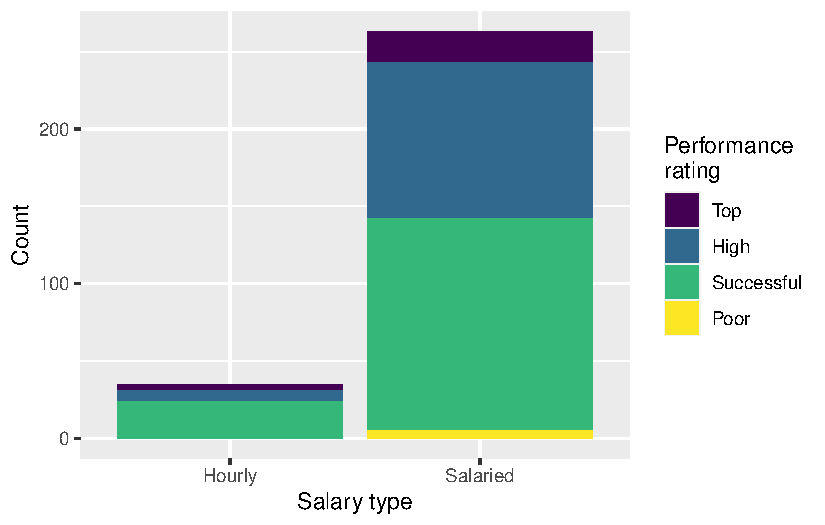
\includegraphics{exam-1-review_files/figure-pdf/fig-salary-performance-rating-1.pdf}

}

}

\subcaption{\label{fig-salary-performance-rating-1}Option 1}
\end{minipage}%
%
\begin{minipage}[t]{0.50\linewidth}

{\centering 

\raisebox{-\height}{

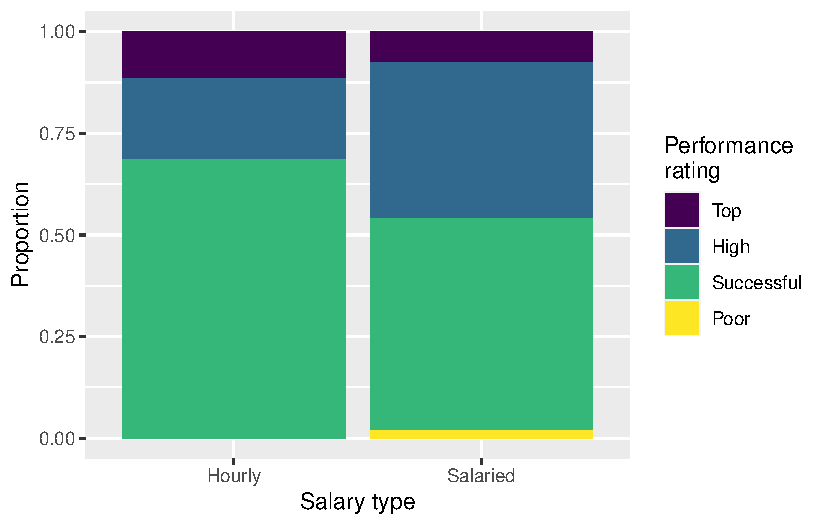
\includegraphics{exam-1-review_files/figure-pdf/fig-salary-performance-rating-2.pdf}

}

}

\subcaption{\label{fig-salary-performance-rating-2}Option 2}
\end{minipage}%

\caption{\label{fig-salary-performance-rating}Distribution of salary
type by performance rating}

\end{figure}

\(\vspace{2cm}\)

\hypertarget{question-11}{%
\subsection{Question 11}\label{question-11}}

A friend with a keen eye points out that the number of observations in
Figure~\ref{fig-salary-performance-rating-1} seems lower than the total
number of observations in \texttt{blizzard\_salary}. What might be going
on here? Explain your reasoning.

\newpage{}

\hypertarget{question-12}{%
\subsection{Question 12}\label{question-12}}

Show the proportions of performance ratings for hourly and salaried
workers in a table and ask students to place those numbers on the
segments of Figure~\ref{fig-salary-performance-rating-2}.

\begin{verbatim}
# A tibble: 4 x 3
  performance_rating Hourly Salaried
  <fct>               <dbl>    <dbl>
1 Successful          0.686   0.521 
2 High                0.2     0.384 
3 Top                 0.114   0.0760
4 Poor                0       0.0190
\end{verbatim}

\hypertarget{question-13}{%
\subsection{Question 13}\label{question-13}}

Figure~\ref{fig-salary-performance-rating-mosaic} is yet another
visualization of the relationship between salary type and performance
rating. What type of plot is ths, and what does it display that
Figure~\ref{fig-salary-performance-rating-2} doesn't?

\begin{figure}

{\centering 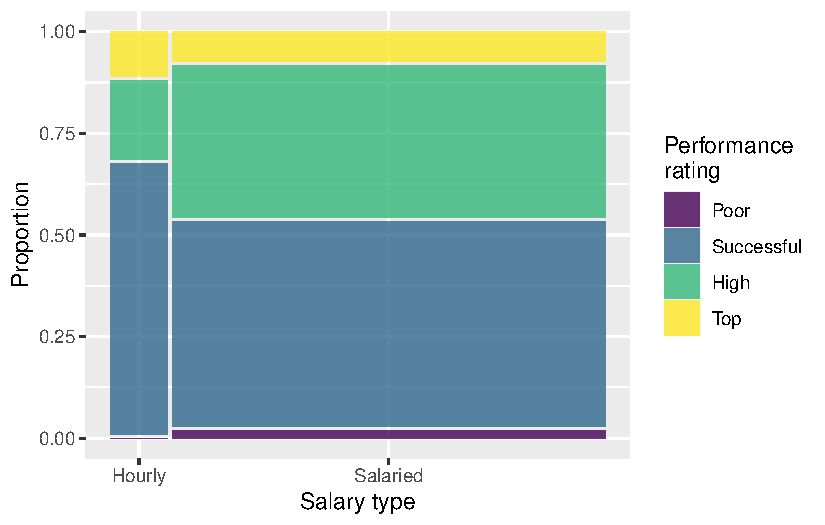
\includegraphics{exam-1-review_files/figure-pdf/fig-salary-performance-rating-mosaic-1.pdf}

}

\caption{\label{fig-salary-performance-rating-mosaic}Another
visualization of salary type by performance rating}

\end{figure}

\(\vspace{2cm}\)

\newpage{}

\hypertarget{question-14}{%
\subsection{Question 14}\label{question-14}}

Suppose we fit a model to predict \texttt{percent\_incr} from
\texttt{annual\_salary} and \texttt{salary\_type}. A tidy output of the
model is shown below.

\begin{verbatim}
# A tibble: 3 x 5
  term                 estimate  std.error statistic p.value
  <chr>                   <dbl>      <dbl>     <dbl>   <dbl>
1 (Intercept)         1.24      0.570           2.18 0.0300 
2 annual_salary       0.0000137 0.00000464      2.96 0.00329
3 salary_typeSalaried 0.913     0.544           1.68 0.0938 
\end{verbatim}

Which of the following visualizations represent this model? Explain your
reasoning.

\begin{figure}

\begin{minipage}[t]{0.50\linewidth}

{\centering 

\raisebox{-\height}{

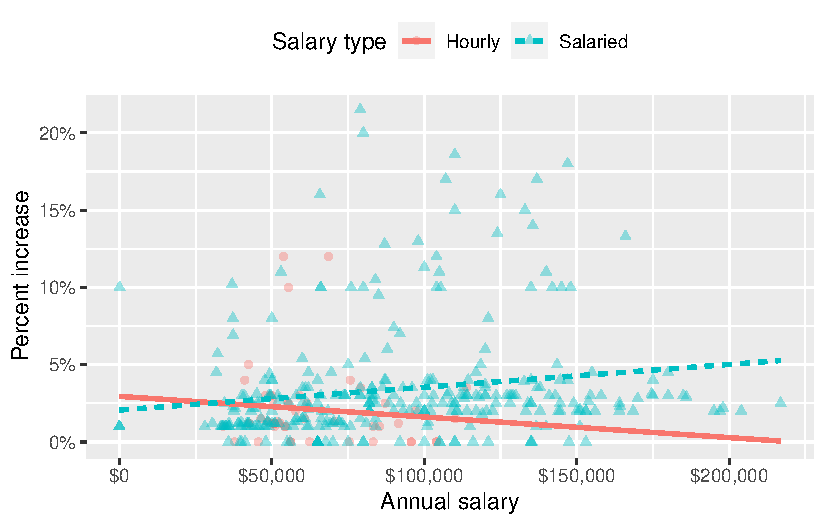
\includegraphics{exam-1-review_files/figure-pdf/fig-raise-salary-type-1.pdf}

}

}

\subcaption{\label{fig-raise-salary-type-1}Option 1}
\end{minipage}%
%
\begin{minipage}[t]{0.50\linewidth}

{\centering 

\raisebox{-\height}{

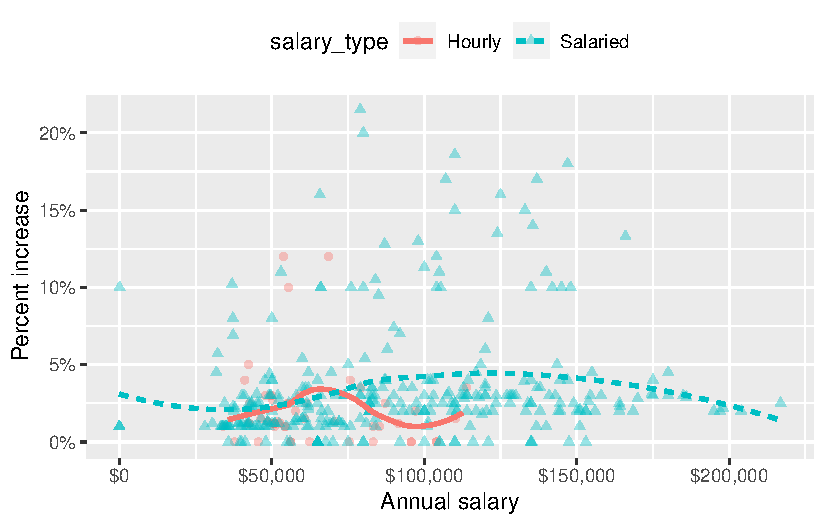
\includegraphics{exam-1-review_files/figure-pdf/fig-raise-salary-type-2.pdf}

}

}

\subcaption{\label{fig-raise-salary-type-2}Option 2}
\end{minipage}%
\newline
\begin{minipage}[t]{0.50\linewidth}

{\centering 

\raisebox{-\height}{

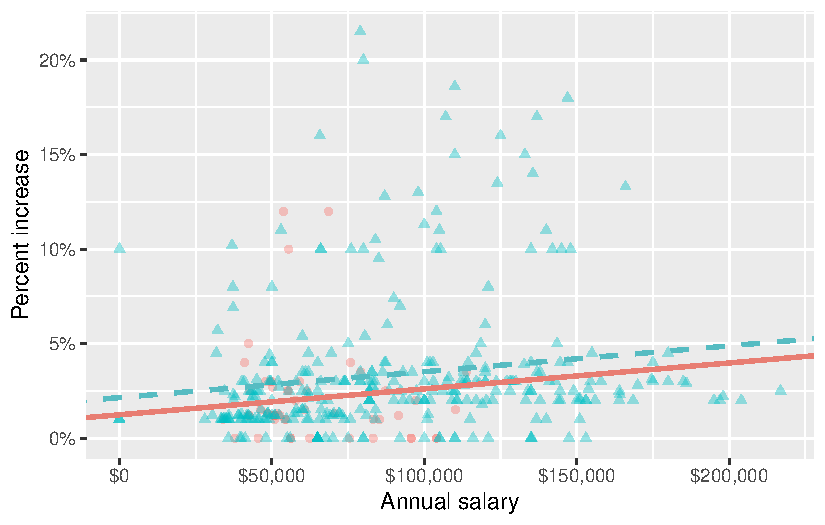
\includegraphics{exam-1-review_files/figure-pdf/fig-raise-salary-type-3.pdf}

}

}

\subcaption{\label{fig-raise-salary-type-3}Option 3}
\end{minipage}%
%
\begin{minipage}[t]{0.50\linewidth}

{\centering 

\raisebox{-\height}{

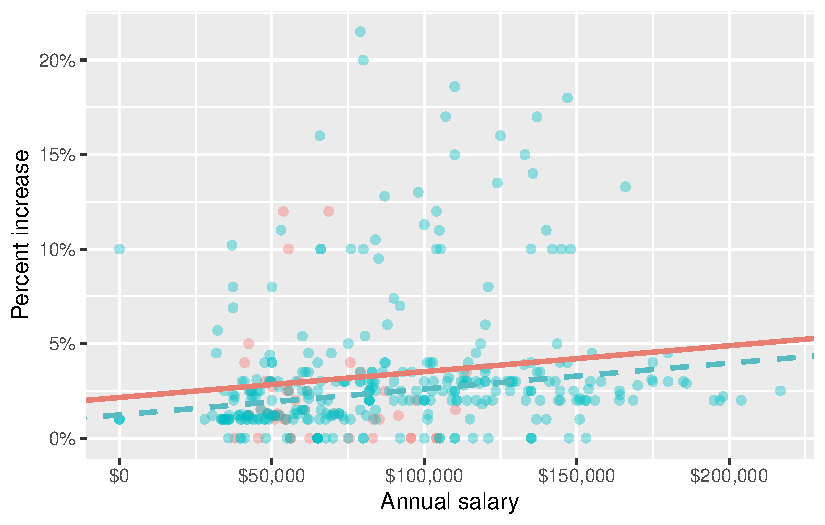
\includegraphics{exam-1-review_files/figure-pdf/fig-raise-salary-type-4.pdf}

}

}

\subcaption{\label{fig-raise-salary-type-4}Option 4}
\end{minipage}%

\caption{\label{fig-raise-salary-type}Visualizations of the relationship
between percent increase, annual salary, and salary type}

\end{figure}

\newpage{}

\hypertarget{question-15}{%
\subsection{Question 15}\label{question-15}}

Define the term parsimonious model.

\(\vspace{2cm}\)

\hypertarget{bonus}{%
\subsection{Bonus}\label{bonus}}

Pick a concept we introduced in class so far that you've been struggling
with and explain it in your own words.

\(\vspace{2cm}\)



\end{document}
